\documentclass{article}
\usepackage[utf8]{inputenc}

\usepackage{tikz}
\usetikzlibrary{positioning, fit}

\begin{document}

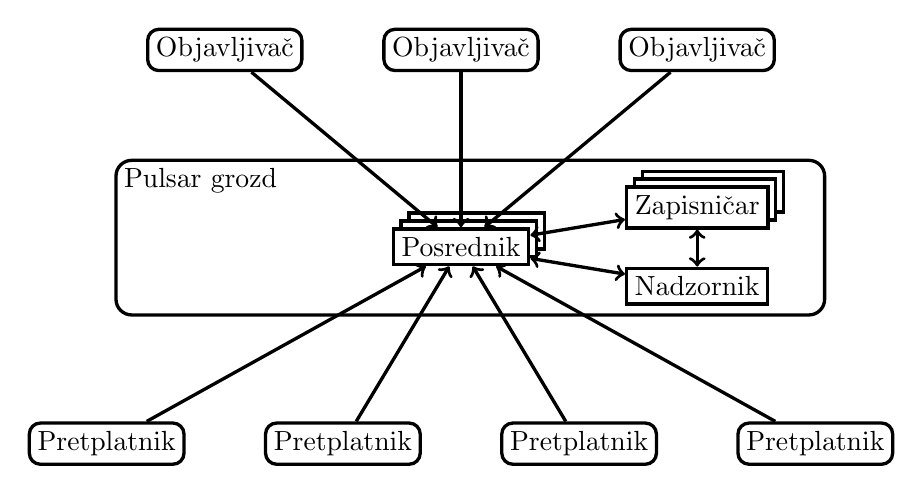
\begin{tikzpicture}[ % has a lot of options; consult the pgf manual
bend angle=45,
long_square/.style={rectangle, draw=black, fill=white, very thick, inner sep=3pt, minimum width=14mm},
rounded_square/.style={rectangle, rounded corners, draw=black, fill=white, very thick, inner sep=3pt, minimum width=14mm},
empty_circle/.style={rectangle, rounded corners=2mm, draw=black, fill=white, very thick, minimum size=4mm},
point/.style={circle, inner sep=0mm},
fit_square/.style={rectangle, rounded corners=2mm, draw=black, very thick, minimum width=90mm},
both_arrow/.style={<->, very thick},
out_arrow/.style={->, very thick},
in_arrow/.style={<-, very thick},
above_edge_text/.style={above, midway, sloped}
]

\node[rounded_square](producer_1) at (1.5,0) {Objavljivač};
\node[rounded_square](producer_2) at (4.5,0) {Objavljivač};
\node[rounded_square](producer_3) at (7.5,0) {Objavljivač};

\node[long_square](bookie_3) at (7.7,-1.8) {Zapisničar};
\node[long_square](bookie_2) at (7.6,-1.9) {Zapisničar};
\node[long_square](bookie_1) at (7.5,-2) {Zapisničar};

\node[long_square](broker_3) at (4.7,-2.3) {Posrednik};
\node[long_square](broker_2) at (4.6,-2.4) {Posrednik};
\node[long_square](broker_1) at (4.5,-2.5) {Posrednik};

\node[long_square](zookeeper) at (7.5,-3) {Nadzornik};

\node[rounded_square](consumer_1) at (0,-5) {Pretplatnik};
\node[rounded_square](consumer_2) at (3,-5) {Pretplatnik};
\node[rounded_square](consumer_3) at (6,-5) {Pretplatnik};
\node[rounded_square](consumer_4) at (9,-5) {Pretplatnik};

\node[fit_square, xshift=-15mm, fit=(bookie_3) (bookie_2) (bookie_1) (broker_3) (broker_2) (broker_1) (zookeeper)] (cluster) {};
\node[anchor=north west] at (cluster.north west) {Pulsar grozd};



\draw[out_arrow](producer_1) to [] node[auto]{} (broker_1);
\draw[out_arrow](producer_2) to [] node[auto]{} (broker_1);
\draw[out_arrow](producer_3) to [] node[auto]{} (broker_1);

\draw[both_arrow](broker_1) to [] node[auto]{} (zookeeper);

\draw[both_arrow](broker_1) to [] node[auto]{} (bookie_1);

\draw[both_arrow](bookie_1) to [] node[auto]{} (zookeeper);

\draw[out_arrow](consumer_1) to [] node[auto]{} (broker_1);
\draw[out_arrow](consumer_2) to [] node[auto]{} (broker_1);
\draw[out_arrow](consumer_3) to [] node[auto]{} (broker_1);
\draw[out_arrow](consumer_4) to [] node[auto]{} (broker_1);

\end{tikzpicture}

\end{document}